\documentclass[1p]{elsarticle_modified}
%\bibliographystyle{elsarticle-num}

%\usepackage[colorlinks]{hyperref}
%\usepackage{abbrmath_seonhwa} %\Abb, \Ascr, \Acal ,\Abf, \Afrak
\usepackage{amsfonts}
\usepackage{amssymb}
\usepackage{amsmath}
\usepackage{amsthm}
\usepackage{scalefnt}
\usepackage{amsbsy}
\usepackage{kotex}
\usepackage{caption}
\usepackage{subfig}
\usepackage{color}
\usepackage{graphicx}
\usepackage{xcolor} %% white, black, red, green, blue, cyan, magenta, yellow
\usepackage{float}
\usepackage{setspace}
\usepackage{hyperref}

\usepackage{tikz}
\usetikzlibrary{arrows}

\usepackage{multirow}
\usepackage{array} % fixed length table
\usepackage{hhline}

%%%%%%%%%%%%%%%%%%%%%
\makeatletter
\renewcommand*\env@matrix[1][\arraystretch]{%
	\edef\arraystretch{#1}%
	\hskip -\arraycolsep
	\let\@ifnextchar\new@ifnextchar
	\array{*\c@MaxMatrixCols c}}
\makeatother %https://tex.stackexchange.com/questions/14071/how-can-i-increase-the-line-spacing-in-a-matrix
%%%%%%%%%%%%%%%

\usepackage[normalem]{ulem}

\newcommand{\msout}[1]{\ifmmode\text{\sout{\ensuremath{#1}}}\else\sout{#1}\fi}
%SOURCE: \msout is \stkout macro in https://tex.stackexchange.com/questions/20609/strikeout-in-math-mode

\newcommand{\cancel}[1]{
	\ifmmode
	{\color{red}\msout{#1}}
	\else
	{\color{red}\sout{#1}}
	\fi
}

\newcommand{\add}[1]{
	{\color{blue}\uwave{#1}}
}

\newcommand{\replace}[2]{
	\ifmmode
	{\color{red}\msout{#1}}{\color{blue}\uwave{#2}}
	\else
	{\color{red}\sout{#1}}{\color{blue}\uwave{#2}}
	\fi
}

\newcommand{\Sol}{\mathcal{S}} %segment
\newcommand{\D}{D} %diagram
\newcommand{\A}{\mathcal{A}} %arc


%%%%%%%%%%%%%%%%%%%%%%%%%%%%%5 test

\def\sl{\operatorname{\textup{SL}}(2,\Cbb)}
\def\psl{\operatorname{\textup{PSL}}(2,\Cbb)}
\def\quan{\mkern 1mu \triangleright \mkern 1mu}

\theoremstyle{definition}
\newtheorem{thm}{Theorem}[section]
\newtheorem{prop}[thm]{Proposition}
\newtheorem{lem}[thm]{Lemma}
\newtheorem{ques}[thm]{Question}
\newtheorem{cor}[thm]{Corollary}
\newtheorem{defn}[thm]{Definition}
\newtheorem{exam}[thm]{Example}
\newtheorem{rmk}[thm]{Remark}
\newtheorem{alg}[thm]{Algorithm}

\newcommand{\I}{\sqrt{-1}}
\begin{document}

%\begin{frontmatter}
%
%\title{Boundary parabolic representations of knots up to 8 crossings}
%
%%% Group authors per affiliation:
%\author{Yunhi Cho} 
%\address{Department of Mathematics, University of Seoul, Seoul, Korea}
%\ead{yhcho@uos.ac.kr}
%
%
%\author{Seonhwa Kim} %\fnref{s_kim}}
%\address{Center for Geometry and Physics, Institute for Basic Science, Pohang, 37673, Korea}
%\ead{ryeona17@ibs.re.kr}
%
%\author{Hyuk Kim}
%\address{Department of Mathematical Sciences, Seoul National University, Seoul 08826, Korea}
%\ead{hyukkim@snu.ac.kr}
%
%\author{Seokbeom Yoon}
%\address{Department of Mathematical Sciences, Seoul National University, Seoul, 08826,  Korea}
%\ead{sbyoon15@snu.ac.kr}
%
%\begin{abstract}
%We find all boundary parabolic representation of knots up to 8 crossings.
%
%\end{abstract}
%\begin{keyword}
%    \MSC[2010] 57M25 
%\end{keyword}
%
%\end{frontmatter}

%\linenumbers
%\tableofcontents
%
\newcommand\colored[1]{\textcolor{white}{\rule[-0.35ex]{0.8em}{1.4ex}}\kern-0.8em\color{red} #1}%
%\newcommand\colored[1]{\textcolor{white}{ #1}\kern-2.17ex	\textcolor{white}{ #1}\kern-1.81ex	\textcolor{white}{ #1}\kern-2.15ex\color{red}#1	}

{\Large $\underline{10_{117}~(K10a_{99})}$}

\setlength{\tabcolsep}{10pt}
\renewcommand{\arraystretch}{1.6}
\vspace{1cm}\begin{tabular}{m{100pt}>{\centering\arraybackslash}m{274pt}}
\multirow{5}{120pt}{
	\centering
	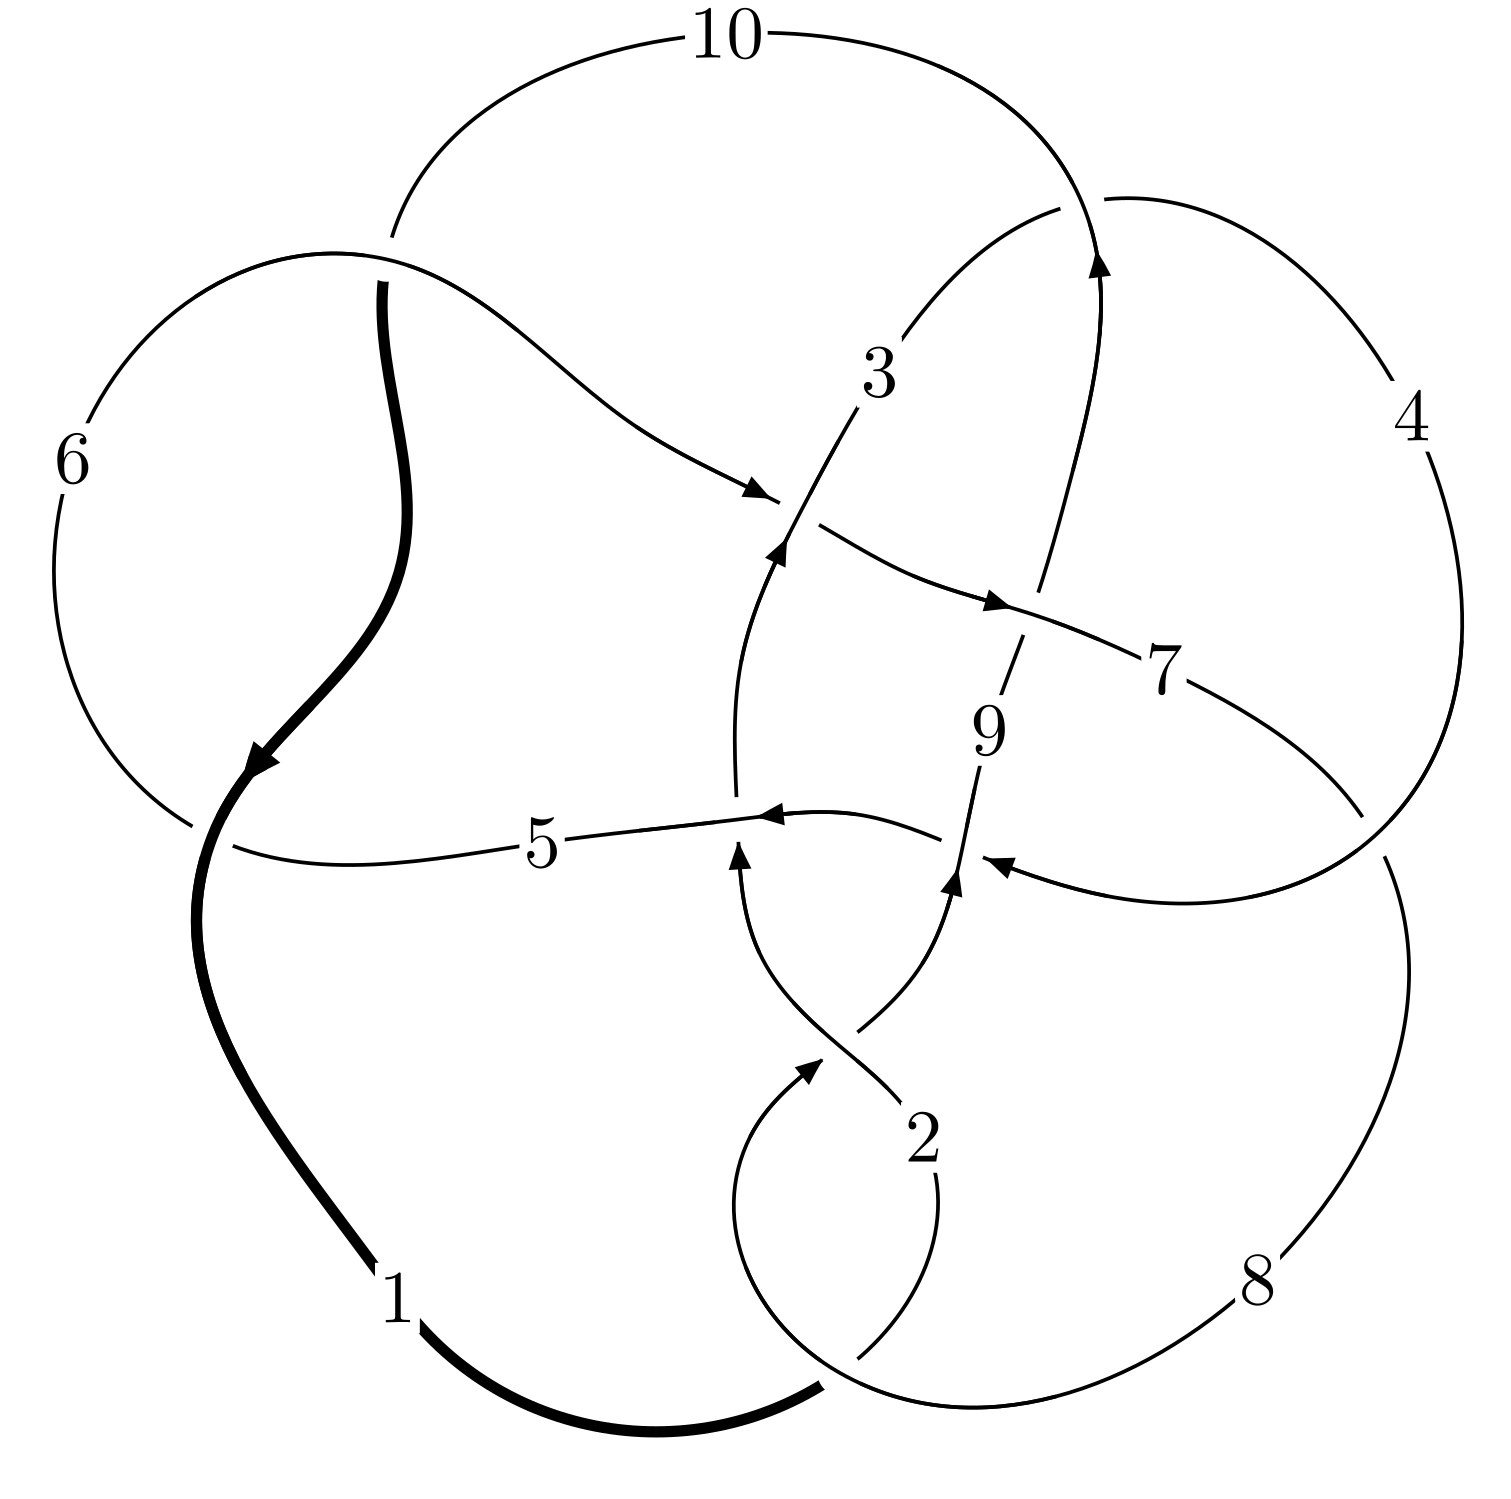
\includegraphics[width=112pt]{../../../GIT/diagram.site/Diagrams/png/201_10_117.png}\\
\ \ \ A knot diagram\footnotemark}&
\allowdisplaybreaks
\textbf{Linearized knot diagam} \\
\cline{2-2}
 &
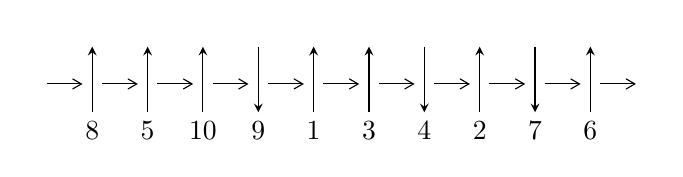
\begin{tikzpicture}[x=20pt, y=17pt]
	% nodes
	\node (C0) at (0, 0) {};
	\node (C1) at (1, 0) {};
	\node (C1U) at (1, +1) {};
	\node (C1D) at (1, -1) {8};

	\node (C2) at (2, 0) {};
	\node (C2U) at (2, +1) {};
	\node (C2D) at (2, -1) {5};

	\node (C3) at (3, 0) {};
	\node (C3U) at (3, +1) {};
	\node (C3D) at (3, -1) {10};

	\node (C4) at (4, 0) {};
	\node (C4U) at (4, +1) {};
	\node (C4D) at (4, -1) {9};

	\node (C5) at (5, 0) {};
	\node (C5U) at (5, +1) {};
	\node (C5D) at (5, -1) {1};

	\node (C6) at (6, 0) {};
	\node (C6U) at (6, +1) {};
	\node (C6D) at (6, -1) {3};

	\node (C7) at (7, 0) {};
	\node (C7U) at (7, +1) {};
	\node (C7D) at (7, -1) {4};

	\node (C8) at (8, 0) {};
	\node (C8U) at (8, +1) {};
	\node (C8D) at (8, -1) {2};

	\node (C9) at (9, 0) {};
	\node (C9U) at (9, +1) {};
	\node (C9D) at (9, -1) {7};

	\node (C10) at (10, 0) {};
	\node (C10U) at (10, +1) {};
	\node (C10D) at (10, -1) {6};
	\node (C11) at (11, 0) {};

	% arrows
	\draw[->,>={angle 60}]
	(C0) edge (C1) (C1) edge (C2) (C2) edge (C3) (C3) edge (C4) (C4) edge (C5) (C5) edge (C6) (C6) edge (C7) (C7) edge (C8) (C8) edge (C9) (C9) edge (C10) (C10) edge (C11) ;	\draw[->,>=stealth]
	(C1D) edge (C1U) (C2D) edge (C2U) (C3D) edge (C3U) (C4U) edge (C4D) (C5D) edge (C5U) (C6D) edge (C6U) (C7U) edge (C7D) (C8D) edge (C8U) (C9U) edge (C9D) (C10D) edge (C10U) ;
	\end{tikzpicture} \\
\hhline{~~} \\& 
\textbf{Solving Sequence} \\ \cline{2-2} 
 &
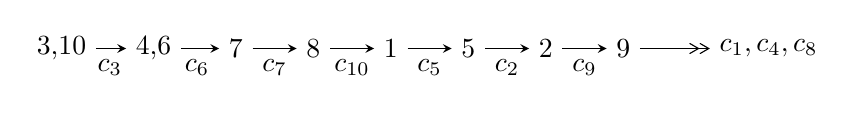
\begin{tikzpicture}[x=28pt, y=7pt]
	% node
	\node (A0) at (-1/8, 0) {3,10};
	\node (A1) at (17/16, 0) {4,6};
	\node (A2) at (17/8, 0) {7};
	\node (A3) at (25/8, 0) {8};
	\node (A4) at (33/8, 0) {1};
	\node (A5) at (41/8, 0) {5};
	\node (A6) at (49/8, 0) {2};
	\node (A7) at (57/8, 0) {9};
	\node (C1) at (1/2, -1) {$c_{3}$};
	\node (C2) at (13/8, -1) {$c_{6}$};
	\node (C3) at (21/8, -1) {$c_{7}$};
	\node (C4) at (29/8, -1) {$c_{10}$};
	\node (C5) at (37/8, -1) {$c_{5}$};
	\node (C6) at (45/8, -1) {$c_{2}$};
	\node (C7) at (53/8, -1) {$c_{9}$};
	\node (A8) at (9, 0) {$c_{1},c_{4},c_{8}$};

	% edge
	\draw[->,>=stealth]	
	(A0) edge (A1) (A1) edge (A2) (A2) edge (A3) (A3) edge (A4) (A4) edge (A5) (A5) edge (A6) (A6) edge (A7) ;
	\draw[->>,>={angle 60}]	
	(A7) edge (A8);
\end{tikzpicture} \\ 

\end{tabular} \\

\footnotetext{
The image of knot diagram is generated by the software ``\textbf{Draw programme}" developed by Andrew Bartholomew(\url{http://www.layer8.co.uk/maths/draw/index.htm\#Running-draw}), where we modified some parts for our purpose(\url{https://github.com/CATsTAILs/LinksPainter}).
}\phantom \\ \newline 
\centering \textbf{Ideals for irreducible components\footnotemark of $X_{\text{par}}$} 
 
\begin{align*}
I^u_{1}&=\langle 
-3.20848\times10^{161} u^{59}+1.04355\times10^{162} u^{58}+\cdots+3.99664\times10^{162} b-4.01482\times10^{162},\\
\phantom{I^u_{1}}&\phantom{= \langle  }5.43983\times10^{162} u^{59}-1.65350\times10^{163} u^{58}+\cdots+3.75684\times10^{163} a+6.18508\times10^{163},\\
\phantom{I^u_{1}}&\phantom{= \langle  }u^{60}-3 u^{59}+\cdots-100 u-47\rangle \\
I^u_{2}&=\langle 
2 u^8+u^7-2 u^6-9 u^5- u^4+u^3-10 u^2+9 b+18 u-5,\\
\phantom{I^u_{2}}&\phantom{= \langle  }-8 u^8-3 u^7-9 u^6+28 u^5-21 u^4+40 u^3-29 u^2+3 a+u-11,\\
\phantom{I^u_{2}}&\phantom{= \langle  }u^9+u^7-4 u^6+4 u^5-6 u^4+6 u^3-2 u^2+2 u-1\rangle \\
\\
\end{align*}
\raggedright * 2 irreducible components of $\dim_{\mathbb{C}}=0$, with total 69 representations.\\
\footnotetext{All coefficients of polynomials are rational numbers. But the coefficients are sometimes approximated in decimal forms when there is not enough margin.}
\newpage
\renewcommand{\arraystretch}{1}
\centering \section*{I. $I^u_{1}= \langle -3.21\times10^{161} u^{59}+1.04\times10^{162} u^{58}+\cdots+4.00\times10^{162} b-4.01\times10^{162},\;5.44\times10^{162} u^{59}-1.65\times10^{163} u^{58}+\cdots+3.76\times10^{163} a+6.19\times10^{163},\;u^{60}-3 u^{59}+\cdots-100 u-47 \rangle$}
\flushleft \textbf{(i) Arc colorings}\\
\begin{tabular}{m{7pt} m{180pt} m{7pt} m{180pt} }
\flushright $a_{3}=$&$\begin{pmatrix}1\\0\end{pmatrix}$ \\
\flushright $a_{10}=$&$\begin{pmatrix}0\\u\end{pmatrix}$ \\
\flushright $a_{4}=$&$\begin{pmatrix}1\\- u^2\end{pmatrix}$ \\
\flushright $a_{6}=$&$\begin{pmatrix}-0.144798 u^{59}+0.440130 u^{58}+\cdots+27.2425 u-1.64635\\0.0802795 u^{59}-0.261107 u^{58}+\cdots-9.37588 u+1.00455\end{pmatrix}$ \\
\flushright $a_{7}=$&$\begin{pmatrix}-0.0645187 u^{59}+0.179024 u^{58}+\cdots+17.8666 u-0.641805\\0.0802795 u^{59}-0.261107 u^{58}+\cdots-9.37588 u+1.00455\end{pmatrix}$ \\
\flushright $a_{8}=$&$\begin{pmatrix}-0.149789 u^{59}+0.442542 u^{58}+\cdots+31.7281 u-0.963328\\0.0559636 u^{59}-0.178921 u^{58}+\cdots-6.13906 u+0.642242\end{pmatrix}$ \\
\flushright $a_{1}=$&$\begin{pmatrix}0.0151173 u^{59}-0.0879877 u^{58}+\cdots+42.0887 u+12.0597\\-0.0276044 u^{59}+0.0511785 u^{58}+\cdots+7.28332 u+2.39479\end{pmatrix}$ \\
\flushright $a_{5}=$&$\begin{pmatrix}0.200110 u^{59}-0.575603 u^{58}+\cdots-63.4707 u+3.83922\\-0.0114669 u^{59}+0.0348903 u^{58}+\cdots+2.13595 u-0.466474\end{pmatrix}$ \\
\flushright $a_{2}=$&$\begin{pmatrix}-0.118992 u^{59}+0.283347 u^{58}+\cdots+73.3930 u+13.4060\\0.0307095 u^{59}-0.111236 u^{58}+\cdots-2.62950 u+1.31233\end{pmatrix}$ \\
\flushright $a_{9}=$&$\begin{pmatrix}-0.0144334 u^{59}-0.0276837 u^{58}+\cdots+46.6833 u+14.8115\\-0.00194635 u^{59}+0.00912555 u^{58}+\cdots-0.688771 u+0.357009\end{pmatrix}$\\&\end{tabular}
\flushleft \textbf{(ii) Obstruction class $= -1$}\\~\\
\flushleft \textbf{(iii) Cusp Shapes $= -0.0308620 u^{59}+0.236254 u^{58}+\cdots-40.3438 u+23.2477$}\\~\\
\newpage\renewcommand{\arraystretch}{1}
\flushleft \textbf{(iv) u-Polynomials at the component}\newline \\
\begin{tabular}{m{50pt}|m{274pt}}
Crossings & \hspace{64pt}u-Polynomials at each crossing \\
\hline $$\begin{aligned}c_{1},c_{8}\end{aligned}$$&$\begin{aligned}
&u^{60}-16 u^{58}+\cdots-24 u+19
\end{aligned}$\\
\hline $$\begin{aligned}c_{2}\end{aligned}$$&$\begin{aligned}
&u^{60}- u^{59}+\cdots-252 u+29
\end{aligned}$\\
\hline $$\begin{aligned}c_{3}\end{aligned}$$&$\begin{aligned}
&u^{60}-3 u^{59}+\cdots-100 u-47
\end{aligned}$\\
\hline $$\begin{aligned}c_{4}\end{aligned}$$&$\begin{aligned}
&u^{60}+u^{59}+\cdots-295 u-37
\end{aligned}$\\
\hline $$\begin{aligned}c_{5},c_{10}\end{aligned}$$&$\begin{aligned}
&u^{60}+u^{59}+\cdots-328 u-49
\end{aligned}$\\
\hline $$\begin{aligned}c_{6}\end{aligned}$$&$\begin{aligned}
&u^{60}+5 u^{58}+\cdots+9 u+1
\end{aligned}$\\
\hline $$\begin{aligned}c_{7}\end{aligned}$$&$\begin{aligned}
&u^{60}+2 u^{59}+\cdots+74 u-19
\end{aligned}$\\
\hline $$\begin{aligned}c_{9}\end{aligned}$$&$\begin{aligned}
&u^{60}-3 u^{59}+\cdots+16 u-1
\end{aligned}$\\
\hline
\end{tabular}\\~\\
\newpage\renewcommand{\arraystretch}{1}
\flushleft \textbf{(v) Riley Polynomials at the component}\newline \\
\begin{tabular}{m{50pt}|m{274pt}}
Crossings & \hspace{64pt}Riley Polynomials at each crossing \\
\hline $$\begin{aligned}c_{1},c_{8}\end{aligned}$$&$\begin{aligned}
&y^{60}-32 y^{59}+\cdots-1602 y+361
\end{aligned}$\\
\hline $$\begin{aligned}c_{2}\end{aligned}$$&$\begin{aligned}
&y^{60}-5 y^{59}+\cdots-61300 y+841
\end{aligned}$\\
\hline $$\begin{aligned}c_{3}\end{aligned}$$&$\begin{aligned}
&y^{60}+13 y^{59}+\cdots+47810 y+2209
\end{aligned}$\\
\hline $$\begin{aligned}c_{4}\end{aligned}$$&$\begin{aligned}
&y^{60}+9 y^{59}+\cdots-29527 y+1369
\end{aligned}$\\
\hline $$\begin{aligned}c_{5},c_{10}\end{aligned}$$&$\begin{aligned}
&y^{60}+37 y^{59}+\cdots+42258 y+2401
\end{aligned}$\\
\hline $$\begin{aligned}c_{6}\end{aligned}$$&$\begin{aligned}
&y^{60}+10 y^{59}+\cdots-45 y+1
\end{aligned}$\\
\hline $$\begin{aligned}c_{7}\end{aligned}$$&$\begin{aligned}
&y^{60}+42 y^{58}+\cdots-7604 y+361
\end{aligned}$\\
\hline $$\begin{aligned}c_{9}\end{aligned}$$&$\begin{aligned}
&y^{60}+y^{59}+\cdots-10 y+1
\end{aligned}$\\
\hline
\end{tabular}\\~\\
\newpage\flushleft \textbf{(vi) Complex Volumes and Cusp Shapes}
$$\begin{array}{c|c|c}  
\text{Solutions to }I^u_{1}& \I (\text{vol} + \sqrt{-1}CS) & \text{Cusp shape}\\
 \hline 
\begin{aligned}
u &= -0.112870 + 0.986911 I \\
a &= -1.159810 + 0.114908 I \\
b &= \phantom{-}0.540790 + 0.509640 I\end{aligned}
 & -3.10319 - 2.00739 I & \phantom{-}0.07017 + 3.73576 I \\ \hline\begin{aligned}
u &= -0.112870 - 0.986911 I \\
a &= -1.159810 - 0.114908 I \\
b &= \phantom{-}0.540790 - 0.509640 I\end{aligned}
 & -3.10319 + 2.00739 I & \phantom{-}0.07017 - 3.73576 I \\ \hline\begin{aligned}
u &= \phantom{-}0.758675 + 0.611167 I \\
a &= \phantom{-}0.595748 - 0.212189 I \\
b &= -0.847394 - 0.210567 I\end{aligned}
 & \phantom{-}1.45806 + 0.40357 I & \phantom{-}7.54100 - 1.19625 I \\ \hline\begin{aligned}
u &= \phantom{-}0.758675 - 0.611167 I \\
a &= \phantom{-}0.595748 + 0.212189 I \\
b &= -0.847394 + 0.210567 I\end{aligned}
 & \phantom{-}1.45806 - 0.40357 I & \phantom{-}7.54100 + 1.19625 I \\ \hline\begin{aligned}
u &= \phantom{-}0.791211 + 0.664753 I \\
a &= \phantom{-}0.043324 + 0.264154 I \\
b &= \phantom{-}0.005931 - 1.204400 I\end{aligned}
 & \phantom{-}1.99327 + 4.92703 I & \phantom{-}6.26354 - 5.97246 I \\ \hline\begin{aligned}
u &= \phantom{-}0.791211 - 0.664753 I \\
a &= \phantom{-}0.043324 - 0.264154 I \\
b &= \phantom{-}0.005931 + 1.204400 I\end{aligned}
 & \phantom{-}1.99327 - 4.92703 I & \phantom{-}6.26354 + 5.97246 I \\ \hline\begin{aligned}
u &= -0.373335 + 0.846791 I \\
a &= -1.34189 + 0.46586 I \\
b &= \phantom{-}1.36952 - 0.80230 I\end{aligned}
 & -3.50470 - 2.65606 I & -0.26583 + 6.15253 I \\ \hline\begin{aligned}
u &= -0.373335 - 0.846791 I \\
a &= -1.34189 - 0.46586 I \\
b &= \phantom{-}1.36952 + 0.80230 I\end{aligned}
 & -3.50470 + 2.65606 I & -0.26583 - 6.15253 I \\ \hline\begin{aligned}
u &= -0.419068 + 0.994844 I \\
a &= -1.154120 + 0.418871 I \\
b &= \phantom{-}0.479030 - 0.178046 I\end{aligned}
 & -3.24917 - 2.13718 I & -0.66405 + 3.46334 I \\ \hline\begin{aligned}
u &= -0.419068 - 0.994844 I \\
a &= -1.154120 - 0.418871 I \\
b &= \phantom{-}0.479030 + 0.178046 I\end{aligned}
 & -3.24917 + 2.13718 I & -0.66405 - 3.46334 I\\
 \hline 
 \end{array}$$\newpage$$\begin{array}{c|c|c}  
\text{Solutions to }I^u_{1}& \I (\text{vol} + \sqrt{-1}CS) & \text{Cusp shape}\\
 \hline 
\begin{aligned}
u &= \phantom{-}0.993764 + 0.432758 I \\
a &= -0.745249 - 0.914388 I \\
b &= \phantom{-}0.92399 + 1.46999 I\end{aligned}
 & \phantom{-}1.75235 + 6.26871 I & \phantom{-}10.64174 - 5.67281 I \\ \hline\begin{aligned}
u &= \phantom{-}0.993764 - 0.432758 I \\
a &= -0.745249 + 0.914388 I \\
b &= \phantom{-}0.92399 - 1.46999 I\end{aligned}
 & \phantom{-}1.75235 - 6.26871 I & \phantom{-}10.64174 + 5.67281 I \\ \hline\begin{aligned}
u &= \phantom{-}0.906827\phantom{ +0.000000I} \\
a &= \phantom{-}0.722755\phantom{ +0.000000I} \\
b &= -0.514151\phantom{ +0.000000I}\end{aligned}
 & \phantom{-}1.17963\phantom{ +0.000000I} & \phantom{-}9.59750\phantom{ +0.000000I} \\ \hline\begin{aligned}
u &= \phantom{-}0.286214 + 0.854751 I \\
a &= \phantom{-}1.69970 - 0.17441 I \\
b &= -0.441193 - 1.061620 I\end{aligned}
 & -1.94749 + 7.99248 I & \phantom{-}0.63462 - 7.50100 I \\ \hline\begin{aligned}
u &= \phantom{-}0.286214 - 0.854751 I \\
a &= \phantom{-}1.69970 + 0.17441 I \\
b &= -0.441193 + 1.061620 I\end{aligned}
 & -1.94749 - 7.99248 I & \phantom{-}0.63462 + 7.50100 I \\ \hline\begin{aligned}
u &= \phantom{-}0.693182 + 0.924086 I \\
a &= -0.459390 + 0.604795 I \\
b &= \phantom{-}0.843186 + 0.654005 I\end{aligned}
 & \phantom{-}0.60848 + 4.96181 I & \phantom{-}4.00000 - 6.29782 I \\ \hline\begin{aligned}
u &= \phantom{-}0.693182 - 0.924086 I \\
a &= -0.459390 - 0.604795 I \\
b &= \phantom{-}0.843186 - 0.654005 I\end{aligned}
 & \phantom{-}0.60848 - 4.96181 I & \phantom{-}4.00000 + 6.29782 I \\ \hline\begin{aligned}
u &= -0.538025 + 0.635820 I \\
a &= \phantom{-}0.059477 + 0.601315 I \\
b &= -0.031984 + 0.666688 I\end{aligned}
 & -1.41050 - 1.53960 I & -1.08247 + 1.71398 I \\ \hline\begin{aligned}
u &= -0.538025 - 0.635820 I \\
a &= \phantom{-}0.059477 - 0.601315 I \\
b &= -0.031984 - 0.666688 I\end{aligned}
 & -1.41050 + 1.53960 I & -1.08247 - 1.71398 I \\ \hline\begin{aligned}
u &= -0.208530 + 0.777299 I \\
a &= \phantom{-}1.54929 + 0.19094 I \\
b &= -0.173386 + 1.263770 I\end{aligned}
 & -4.80506 - 1.60983 I & -3.59396 + 7.39228 I\\
 \hline 
 \end{array}$$\newpage$$\begin{array}{c|c|c}  
\text{Solutions to }I^u_{1}& \I (\text{vol} + \sqrt{-1}CS) & \text{Cusp shape}\\
 \hline 
\begin{aligned}
u &= -0.208530 - 0.777299 I \\
a &= \phantom{-}1.54929 - 0.19094 I \\
b &= -0.173386 - 1.263770 I\end{aligned}
 & -4.80506 + 1.60983 I & -3.59396 - 7.39228 I \\ \hline\begin{aligned}
u &= \phantom{-}0.824128 + 0.877490 I \\
a &= \phantom{-}0.878482 + 0.225172 I \\
b &= -0.96089 - 1.31598 I\end{aligned}
 & \phantom{-}3.14073 + 5.21448 I & \phantom{-0.000000 } 0 \\ \hline\begin{aligned}
u &= \phantom{-}0.824128 - 0.877490 I \\
a &= \phantom{-}0.878482 - 0.225172 I \\
b &= -0.96089 + 1.31598 I\end{aligned}
 & \phantom{-}3.14073 - 5.21448 I & \phantom{-0.000000 } 0 \\ \hline\begin{aligned}
u &= -0.521047 + 0.599991 I \\
a &= -0.246524 - 1.324130 I \\
b &= \phantom{-}0.819658 - 0.613048 I\end{aligned}
 & \phantom{-}4.56427 + 0.06184 I & \phantom{-}9.79376 + 2.89093 I \\ \hline\begin{aligned}
u &= -0.521047 - 0.599991 I \\
a &= -0.246524 + 1.324130 I \\
b &= \phantom{-}0.819658 + 0.613048 I\end{aligned}
 & \phantom{-}4.56427 - 0.06184 I & \phantom{-}9.79376 - 2.89093 I \\ \hline\begin{aligned}
u &= -0.911068 + 0.857587 I \\
a &= -0.800663 - 0.622002 I \\
b &= \phantom{-}0.887791 - 0.659627 I\end{aligned}
 & \phantom{-}4.45627 - 9.81230 I & \phantom{-0.000000 } 0 \\ \hline\begin{aligned}
u &= -0.911068 - 0.857587 I \\
a &= -0.800663 + 0.622002 I \\
b &= \phantom{-}0.887791 + 0.659627 I\end{aligned}
 & \phantom{-}4.45627 + 9.81230 I & \phantom{-0.000000 } 0 \\ \hline\begin{aligned}
u &= \phantom{-}0.520353 + 0.534999 I \\
a &= \phantom{-}1.60615 - 0.69113 I \\
b &= -0.244986 - 0.494041 I\end{aligned}
 & \phantom{-}1.62697 - 0.89360 I & \phantom{-}2.00328 - 3.90798 I \\ \hline\begin{aligned}
u &= \phantom{-}0.520353 - 0.534999 I \\
a &= \phantom{-}1.60615 + 0.69113 I \\
b &= -0.244986 + 0.494041 I\end{aligned}
 & \phantom{-}1.62697 + 0.89360 I & \phantom{-}2.00328 + 3.90798 I \\ \hline\begin{aligned}
u &= -1.242100 + 0.227160 I \\
a &= -0.033020 - 0.829489 I \\
b &= \phantom{-}0.352953 + 0.262356 I\end{aligned}
 & -0.86533 + 2.68701 I & \phantom{-0.000000 } 0\\
 \hline 
 \end{array}$$\newpage$$\begin{array}{c|c|c}  
\text{Solutions to }I^u_{1}& \I (\text{vol} + \sqrt{-1}CS) & \text{Cusp shape}\\
 \hline 
\begin{aligned}
u &= -1.242100 - 0.227160 I \\
a &= -0.033020 + 0.829489 I \\
b &= \phantom{-}0.352953 - 0.262356 I\end{aligned}
 & -0.86533 - 2.68701 I & \phantom{-0.000000 } 0 \\ \hline\begin{aligned}
u &= -0.282250 + 0.670079 I \\
a &= \phantom{-}1.37086 - 0.50401 I \\
b &= -0.81149 + 1.93630 I\end{aligned}
 & -4.32803 - 0.39404 I & -0.42763 - 3.09033 I \\ \hline\begin{aligned}
u &= -0.282250 - 0.670079 I \\
a &= \phantom{-}1.37086 + 0.50401 I \\
b &= -0.81149 - 1.93630 I\end{aligned}
 & -4.32803 + 0.39404 I & -0.42763 + 3.09033 I \\ \hline\begin{aligned}
u &= \phantom{-}0.775420 + 1.016880 I \\
a &= \phantom{-}0.283940 + 0.475986 I \\
b &= \phantom{-}0.385422 - 0.306091 I\end{aligned}
 & \phantom{-}2.81417 + 0.85474 I & \phantom{-0.000000 } 0 \\ \hline\begin{aligned}
u &= \phantom{-}0.775420 - 1.016880 I \\
a &= \phantom{-}0.283940 - 0.475986 I \\
b &= \phantom{-}0.385422 + 0.306091 I\end{aligned}
 & \phantom{-}2.81417 - 0.85474 I & \phantom{-0.000000 } 0 \\ \hline\begin{aligned}
u &= -0.654495 + 0.222235 I \\
a &= \phantom{-}0.913613 + 0.492134 I \\
b &= -1.171170 + 0.662981 I\end{aligned}
 & \phantom{-}5.22239 - 2.37989 I & \phantom{-}14.0342 + 3.0404 I \\ \hline\begin{aligned}
u &= -0.654495 - 0.222235 I \\
a &= \phantom{-}0.913613 - 0.492134 I \\
b &= -1.171170 - 0.662981 I\end{aligned}
 & \phantom{-}5.22239 + 2.37989 I & \phantom{-}14.0342 - 3.0404 I \\ \hline\begin{aligned}
u &= \phantom{-}0.008423 + 0.554656 I \\
a &= \phantom{-}2.05543 + 0.36150 I \\
b &= -1.23945 - 1.72511 I\end{aligned}
 & -0.66314 - 6.63784 I & -0.93799 + 7.96550 I \\ \hline\begin{aligned}
u &= \phantom{-}0.008423 - 0.554656 I \\
a &= \phantom{-}2.05543 - 0.36150 I \\
b &= -1.23945 + 1.72511 I\end{aligned}
 & -0.66314 + 6.63784 I & -0.93799 - 7.96550 I \\ \hline\begin{aligned}
u &= -0.82689 + 1.22977 I \\
a &= \phantom{-}0.911137 - 0.237809 I \\
b &= -1.19326 + 1.23882 I\end{aligned}
 & -3.51043 - 9.84939 I & \phantom{-0.000000 } 0\\
 \hline 
 \end{array}$$\newpage$$\begin{array}{c|c|c}  
\text{Solutions to }I^u_{1}& \I (\text{vol} + \sqrt{-1}CS) & \text{Cusp shape}\\
 \hline 
\begin{aligned}
u &= -0.82689 - 1.22977 I \\
a &= \phantom{-}0.911137 + 0.237809 I \\
b &= -1.19326 - 1.23882 I\end{aligned}
 & -3.51043 + 9.84939 I & \phantom{-0.000000 } 0 \\ \hline\begin{aligned}
u &= -0.81360 + 1.26582 I \\
a &= -0.915368 + 0.302763 I \\
b &= \phantom{-}0.929673 - 0.916332 I\end{aligned}
 & -4.28857 - 3.85212 I & \phantom{-0.000000 } 0 \\ \hline\begin{aligned}
u &= -0.81360 - 1.26582 I \\
a &= -0.915368 - 0.302763 I \\
b &= \phantom{-}0.929673 + 0.916332 I\end{aligned}
 & -4.28857 + 3.85212 I & \phantom{-0.000000 } 0 \\ \hline\begin{aligned}
u &= -0.469315\phantom{ +0.000000I} \\
a &= \phantom{-}5.77453\phantom{ +0.000000I} \\
b &= -0.184074\phantom{ +0.000000I}\end{aligned}
 & -0.389771\phantom{ +0.000000I} & \phantom{-}203.390\phantom{ +0.000000I} \\ \hline\begin{aligned}
u &= -0.07505 + 1.52982 I \\
a &= \phantom{-}0.651890 + 0.069835 I \\
b &= -1.327120 - 0.173804 I\end{aligned}
 & \phantom{-}2.01747 - 2.78040 I & \phantom{-0.000000 } 0 \\ \hline\begin{aligned}
u &= -0.07505 - 1.52982 I \\
a &= \phantom{-}0.651890 - 0.069835 I \\
b &= -1.327120 + 0.173804 I\end{aligned}
 & \phantom{-}2.01747 + 2.78040 I & \phantom{-0.000000 } 0 \\ \hline\begin{aligned}
u &= -0.93774 + 1.26399 I \\
a &= \phantom{-}0.536599 + 0.151412 I \\
b &= -0.870982 - 0.095094 I\end{aligned}
 & \phantom{-}3.61034 + 3.01624 I & \phantom{-0.000000 } 0 \\ \hline\begin{aligned}
u &= -0.93774 - 1.26399 I \\
a &= \phantom{-}0.536599 - 0.151412 I \\
b &= -0.870982 + 0.095094 I\end{aligned}
 & \phantom{-}3.61034 - 3.01624 I & \phantom{-0.000000 } 0 \\ \hline\begin{aligned}
u &= \phantom{-}0.047283 + 0.408643 I \\
a &= -4.41257 - 0.03304 I \\
b &= \phantom{-}0.656591 - 0.103431 I\end{aligned}
 & -0.647397 + 0.825379 I & \phantom{-}13.47557 + 3.84496 I \\ \hline\begin{aligned}
u &= \phantom{-}0.047283 - 0.408643 I \\
a &= -4.41257 + 0.03304 I \\
b &= \phantom{-}0.656591 + 0.103431 I\end{aligned}
 & -0.647397 - 0.825379 I & \phantom{-}13.47557 - 3.84496 I\\
 \hline 
 \end{array}$$\newpage$$\begin{array}{c|c|c}  
\text{Solutions to }I^u_{1}& \I (\text{vol} + \sqrt{-1}CS) & \text{Cusp shape}\\
 \hline 
\begin{aligned}
u &= \phantom{-}0.96616 + 1.29625 I \\
a &= \phantom{-}0.917595 + 0.250498 I \\
b &= -1.16052 - 1.17459 I\end{aligned}
 & -0.3709 + 16.1254 I & \phantom{-0.000000 } 0 \\ \hline\begin{aligned}
u &= \phantom{-}0.96616 - 1.29625 I \\
a &= \phantom{-}0.917595 - 0.250498 I \\
b &= -1.16052 + 1.17459 I\end{aligned}
 & -0.3709 - 16.1254 I & \phantom{-0.000000 } 0 \\ \hline\begin{aligned}
u &= \phantom{-}0.92727 + 1.34544 I \\
a &= -0.868668 - 0.126514 I \\
b &= \phantom{-}0.891724 + 0.853255 I\end{aligned}
 & -3.18307 + 7.41862 I & \phantom{-0.000000 } 0 \\ \hline\begin{aligned}
u &= \phantom{-}0.92727 - 1.34544 I \\
a &= -0.868668 + 0.126514 I \\
b &= \phantom{-}0.891724 - 0.853255 I\end{aligned}
 & -3.18307 - 7.41862 I & \phantom{-0.000000 } 0 \\ \hline\begin{aligned}
u &= -1.23044 + 1.25774 I \\
a &= -0.588762 + 0.477885 I \\
b &= \phantom{-}0.728116 - 1.050760 I\end{aligned}
 & -2.92948 - 5.60961 I & \phantom{-0.000000 } 0 \\ \hline\begin{aligned}
u &= -1.23044 - 1.25774 I \\
a &= -0.588762 - 0.477885 I \\
b &= \phantom{-}0.728116 + 1.050760 I\end{aligned}
 & -2.92948 + 5.60961 I & \phantom{-0.000000 } 0 \\ \hline\begin{aligned}
u &= \phantom{-}1.02141 + 1.47167 I \\
a &= -0.494856 - 0.297340 I \\
b &= \phantom{-}0.694021 + 0.906910 I\end{aligned}
 & -2.63315 + 3.07819 I & \phantom{-0.000000 } 0 \\ \hline\begin{aligned}
u &= \phantom{-}1.02141 - 1.47167 I \\
a &= -0.494856 + 0.297340 I \\
b &= \phantom{-}0.694021 - 0.906910 I\end{aligned}
 & -2.63315 - 3.07819 I & \phantom{-0.000000 } 0 \\ \hline\begin{aligned}
u &= \phantom{-}1.81425 + 0.48435 I \\
a &= -0.069087 + 0.592288 I \\
b &= \phantom{-}0.314536 - 0.264463 I\end{aligned}
 & \phantom{-}2.02262 - 7.30145 I & \phantom{-0.000000 } 0 \\ \hline\begin{aligned}
u &= \phantom{-}1.81425 - 0.48435 I \\
a &= -0.069087 - 0.592288 I \\
b &= \phantom{-}0.314536 + 0.264463 I\end{aligned}
 & \phantom{-}2.02262 + 7.30145 I & \phantom{-0.000000 } 0\\
 \hline 
 \end{array}$$\newpage\newpage\renewcommand{\arraystretch}{1}
\centering \section*{II. $I^u_{2}= \langle 2 u^8+u^7+\cdots+9 b-5,\;-8 u^8-3 u^7+\cdots+3 a-11,\;u^9+u^7+\cdots+2 u-1 \rangle$}
\flushleft \textbf{(i) Arc colorings}\\
\begin{tabular}{m{7pt} m{180pt} m{7pt} m{180pt} }
\flushright $a_{3}=$&$\begin{pmatrix}1\\0\end{pmatrix}$ \\
\flushright $a_{10}=$&$\begin{pmatrix}0\\u\end{pmatrix}$ \\
\flushright $a_{4}=$&$\begin{pmatrix}1\\- u^2\end{pmatrix}$ \\
\flushright $a_{6}=$&$\begin{pmatrix}\frac{8}{3} u^8+u^7+\cdots-\frac{1}{3} u+\frac{11}{3}\\-\frac{2}{9} u^8-\frac{1}{9} u^7+\cdots-2 u+\frac{5}{9}\end{pmatrix}$ \\
\flushright $a_{7}=$&$\begin{pmatrix}\frac{22}{9} u^8+\frac{8}{9} u^7+\cdots-\frac{7}{3} u+\frac{38}{9}\\-\frac{2}{9} u^8-\frac{1}{9} u^7+\cdots-2 u+\frac{5}{9}\end{pmatrix}$ \\
\flushright $a_{8}=$&$\begin{pmatrix}\frac{17}{9} u^8+\frac{4}{9} u^7+\cdots- u+\frac{25}{9}\\\frac{1}{3} u^8+\frac{1}{3} u^7+\cdots-\frac{7}{3} u+1\end{pmatrix}$ \\
\flushright $a_{1}=$&$\begin{pmatrix}\frac{46}{9} u^8+\frac{29}{9} u^7+\cdots+\frac{5}{3} u+\frac{77}{9}\\\frac{1}{9} u^8-\frac{7}{9} u^7+\cdots-\frac{1}{3} u-\frac{4}{9}\end{pmatrix}$ \\
\flushright $a_{5}=$&$\begin{pmatrix}\frac{119}{9} u^8+\frac{64}{9} u^7+\cdots- u+\frac{229}{9}\\\frac{1}{3} u^8+\frac{1}{3} u^7+\cdots+\frac{1}{3} u^2+\frac{2}{3} u\end{pmatrix}$ \\
\flushright $a_{2}=$&$\begin{pmatrix}\frac{32}{9} u^8+\frac{16}{9} u^7+\cdots- u+\frac{64}{9}\\\frac{2}{9} u^8+\frac{1}{9} u^7+\cdots- u+\frac{4}{9}\end{pmatrix}$ \\
\flushright $a_{9}=$&$\begin{pmatrix}\frac{46}{9} u^8+\frac{17}{9} u^7+\cdots-\frac{8}{3} u+\frac{80}{9}\\-\frac{1}{9} u^8-\frac{5}{9} u^7+\cdots-2 u+\frac{7}{9}\end{pmatrix}$\\&\end{tabular}
\flushleft \textbf{(ii) Obstruction class $= 1$}\\~\\
\flushleft \textbf{(iii) Cusp Shapes $= -\frac{454}{9} u^8-\frac{245}{9} u^7-\frac{599}{9} u^6+166 u^5-\frac{1024}{9} u^4+\frac{2203}{9} u^3-\frac{1618}{9} u^2+13 u-\frac{845}{9}$}\\~\\
\newpage\renewcommand{\arraystretch}{1}
\flushleft \textbf{(iv) u-Polynomials at the component}\newline \\
\begin{tabular}{m{50pt}|m{274pt}}
Crossings & \hspace{64pt}u-Polynomials at each crossing \\
\hline $$\begin{aligned}c_{1}\end{aligned}$$&$\begin{aligned}
&u^9+u^8- u^7- u^6- u^5- u^4+4 u^3+2 u^2-2 u-1
\end{aligned}$\\
\hline $$\begin{aligned}c_{2}\end{aligned}$$&$\begin{aligned}
&u^9+4 u^8+10 u^7+20 u^6+34 u^5+42 u^4+30 u^3+9 u^2-1
\end{aligned}$\\
\hline $$\begin{aligned}c_{3}\end{aligned}$$&$\begin{aligned}
&u^9+u^7-4 u^6+4 u^5-6 u^4+6 u^3-2 u^2+2 u-1
\end{aligned}$\\
\hline $$\begin{aligned}c_{4}\end{aligned}$$&$\begin{aligned}
&u^9-2 u^8- u^7-3 u^6-3 u^5-5 u^3-4 u^2- u-1
\end{aligned}$\\
\hline $$\begin{aligned}c_{5}\end{aligned}$$&$\begin{aligned}
&u^9-2 u^8+3 u^7-7 u^6+u^5-10 u^4-4 u^3-6 u^2-4 u-1
\end{aligned}$\\
\hline $$\begin{aligned}c_{6}\end{aligned}$$&$\begin{aligned}
&u^9+u^8+4 u^7- u^6+u^5-8 u^4-3 u^2+7 u-1
\end{aligned}$\\
\hline $$\begin{aligned}c_{7}\end{aligned}$$&$\begin{aligned}
&u^9- u^8+3 u^7+u^6+u^5+3 u^4+3 u^3+5 u^2+1
\end{aligned}$\\
\hline $$\begin{aligned}c_{8}\end{aligned}$$&$\begin{aligned}
&u^9- u^8- u^7+u^6- u^5+u^4+4 u^3-2 u^2-2 u+1
\end{aligned}$\\
\hline $$\begin{aligned}c_{9}\end{aligned}$$&$\begin{aligned}
&u^9+4 u^8+5 u^7+3 u^6+2 u^5+2 u^4+u^3+1
\end{aligned}$\\
\hline $$\begin{aligned}c_{10}\end{aligned}$$&$\begin{aligned}
&u^9+2 u^8+3 u^7+7 u^6+u^5+10 u^4-4 u^3+6 u^2-4 u+1
\end{aligned}$\\
\hline
\end{tabular}\\~\\
\newpage\renewcommand{\arraystretch}{1}
\flushleft \textbf{(v) Riley Polynomials at the component}\newline \\
\begin{tabular}{m{50pt}|m{274pt}}
Crossings & \hspace{64pt}Riley Polynomials at each crossing \\
\hline $$\begin{aligned}c_{1},c_{8}\end{aligned}$$&$\begin{aligned}
&y^9-3 y^8+y^7+11 y^6-17 y^5+y^4+22 y^3-22 y^2+8 y-1
\end{aligned}$\\
\hline $$\begin{aligned}c_{2}\end{aligned}$$&$\begin{aligned}
&y^9+4 y^8+8 y^7+4 y^6+4 y^5-76 y^4+184 y^3+3 y^2+18 y-1
\end{aligned}$\\
\hline $$\begin{aligned}c_{3}\end{aligned}$$&$\begin{aligned}
&y^9+2 y^8+9 y^7+4 y^6-16 y^5+20 y^3+8 y^2-1
\end{aligned}$\\
\hline $$\begin{aligned}c_{4}\end{aligned}$$&$\begin{aligned}
&y^9-6 y^8-17 y^7-13 y^6+y^5+4 y^4+25 y^3-6 y^2-7 y-1
\end{aligned}$\\
\hline $$\begin{aligned}c_{5},c_{10}\end{aligned}$$&$\begin{aligned}
&y^9+2 y^8-17 y^7-91 y^6-195 y^5-220 y^4-126 y^3-24 y^2+4 y-1
\end{aligned}$\\
\hline $$\begin{aligned}c_{6}\end{aligned}$$&$\begin{aligned}
&y^9+7 y^8+20 y^7+23 y^6+5 y^5-12 y^4-36 y^3-25 y^2+43 y-1
\end{aligned}$\\
\hline $$\begin{aligned}c_{7}\end{aligned}$$&$\begin{aligned}
&y^9+5 y^8+13 y^7+17 y^6+23 y^5-11 y^4-23 y^3-31 y^2-10 y-1
\end{aligned}$\\
\hline $$\begin{aligned}c_{9}\end{aligned}$$&$\begin{aligned}
&y^9-6 y^8+5 y^7-3 y^6+2 y^5-8 y^4-5 y^3-4 y^2-1
\end{aligned}$\\
\hline
\end{tabular}\\~\\
\newpage\flushleft \textbf{(vi) Complex Volumes and Cusp Shapes}
$$\begin{array}{c|c|c}  
\text{Solutions to }I^u_{2}& \I (\text{vol} + \sqrt{-1}CS) & \text{Cusp shape}\\
 \hline 
\begin{aligned}
u &= \phantom{-}0.055585 + 1.071070 I \\
a &= \phantom{-}0.151372 + 0.325268 I \\
b &= -0.911604 - 0.103130 I\end{aligned}
 & \phantom{-}3.57395 + 1.78451 I & \phantom{-}10.19091 - 0.99326 I \\ \hline\begin{aligned}
u &= \phantom{-}0.055585 - 1.071070 I \\
a &= \phantom{-}0.151372 - 0.325268 I \\
b &= -0.911604 + 0.103130 I\end{aligned}
 & \phantom{-}3.57395 - 1.78451 I & \phantom{-}10.19091 + 0.99326 I \\ \hline\begin{aligned}
u &= \phantom{-}1.040640 + 0.285855 I \\
a &= -0.561905 - 0.895180 I \\
b &= \phantom{-}0.161935 + 1.373030 I\end{aligned}
 & \phantom{-}0.72688 + 6.70635 I & \phantom{-}3.06894 - 7.87674 I \\ \hline\begin{aligned}
u &= \phantom{-}1.040640 - 0.285855 I \\
a &= -0.561905 + 0.895180 I \\
b &= \phantom{-}0.161935 - 1.373030 I\end{aligned}
 & \phantom{-}0.72688 - 6.70635 I & \phantom{-}3.06894 + 7.87674 I \\ \hline\begin{aligned}
u &= -0.244831 + 0.626842 I \\
a &= -1.67953 + 0.25795 I \\
b &= \phantom{-}0.53282 - 1.62052 I\end{aligned}
 & -4.15988 - 1.15529 I & \phantom{-}3.41918 + 3.86401 I \\ \hline\begin{aligned}
u &= -0.244831 - 0.626842 I \\
a &= -1.67953 - 0.25795 I \\
b &= \phantom{-}0.53282 + 1.62052 I\end{aligned}
 & -4.15988 + 1.15529 I & \phantom{-}3.41918 - 3.86401 I \\ \hline\begin{aligned}
u &= \phantom{-}0.524555\phantom{ +0.000000I} \\
a &= \phantom{-}4.47522\phantom{ +0.000000I} \\
b &= -0.153592\phantom{ +0.000000I}\end{aligned}
 & -0.416370\phantom{ +0.000000I} & -105.200\phantom{ +0.000000I} \\ \hline\begin{aligned}
u &= -1.11367 + 1.37911 I \\
a &= -0.647547 + 0.344854 I \\
b &= \phantom{-}0.793645 - 0.872272 I\end{aligned}
 & -3.22264 - 4.71392 I & \phantom{-}2.42181 + 4.00779 I \\ \hline\begin{aligned}
u &= -1.11367 - 1.37911 I \\
a &= -0.647547 - 0.344854 I \\
b &= \phantom{-}0.793645 + 0.872272 I\end{aligned}
 & -3.22264 + 4.71392 I & \phantom{-}2.42181 - 4.00779 I\\
 \hline 
 \end{array}$$\newpage
\newpage\renewcommand{\arraystretch}{1}
\centering \section*{ III. u-Polynomials}
\begin{tabular}{m{50pt}|m{274pt}}
Crossings & \hspace{64pt}u-Polynomials at each crossing \\
\hline $$\begin{aligned}c_{1}\end{aligned}$$&$\begin{aligned}
&(u^9+u^8- u^7- u^6- u^5- u^4+4 u^3+2 u^2-2 u-1)\\
&\cdot(u^{60}-16 u^{58}+\cdots-24 u+19)
\end{aligned}$\\
\hline $$\begin{aligned}c_{2}\end{aligned}$$&$\begin{aligned}
&(u^9+4 u^8+10 u^7+20 u^6+34 u^5+42 u^4+30 u^3+9 u^2-1)\\
&\cdot(u^{60}- u^{59}+\cdots-252 u+29)
\end{aligned}$\\
\hline $$\begin{aligned}c_{3}\end{aligned}$$&$\begin{aligned}
&(u^9+u^7-4 u^6+4 u^5-6 u^4+6 u^3-2 u^2+2 u-1)\\
&\cdot(u^{60}-3 u^{59}+\cdots-100 u-47)
\end{aligned}$\\
\hline $$\begin{aligned}c_{4}\end{aligned}$$&$\begin{aligned}
&(u^9-2 u^8- u^7-3 u^6-3 u^5-5 u^3-4 u^2- u-1)\\
&\cdot(u^{60}+u^{59}+\cdots-295 u-37)
\end{aligned}$\\
\hline $$\begin{aligned}c_{5}\end{aligned}$$&$\begin{aligned}
&(u^9-2 u^8+3 u^7-7 u^6+u^5-10 u^4-4 u^3-6 u^2-4 u-1)\\
&\cdot(u^{60}+u^{59}+\cdots-328 u-49)
\end{aligned}$\\
\hline $$\begin{aligned}c_{6}\end{aligned}$$&$\begin{aligned}
&(u^9+u^8+\cdots+7 u-1)(u^{60}+5 u^{58}+\cdots+9 u+1)
\end{aligned}$\\
\hline $$\begin{aligned}c_{7}\end{aligned}$$&$\begin{aligned}
&(u^9- u^8+3 u^7+u^6+u^5+3 u^4+3 u^3+5 u^2+1)\\
&\cdot(u^{60}+2 u^{59}+\cdots+74 u-19)
\end{aligned}$\\
\hline $$\begin{aligned}c_{8}\end{aligned}$$&$\begin{aligned}
&(u^9- u^8- u^7+u^6- u^5+u^4+4 u^3-2 u^2-2 u+1)\\
&\cdot(u^{60}-16 u^{58}+\cdots-24 u+19)
\end{aligned}$\\
\hline $$\begin{aligned}c_{9}\end{aligned}$$&$\begin{aligned}
&(u^9+4 u^8+\cdots+u^3+1)(u^{60}-3 u^{59}+\cdots+16 u-1)
\end{aligned}$\\
\hline $$\begin{aligned}c_{10}\end{aligned}$$&$\begin{aligned}
&(u^9+2 u^8+3 u^7+7 u^6+u^5+10 u^4-4 u^3+6 u^2-4 u+1)\\
&\cdot(u^{60}+u^{59}+\cdots-328 u-49)
\end{aligned}$\\
\hline
\end{tabular}\newpage\renewcommand{\arraystretch}{1}
\centering \section*{ IV. Riley Polynomials}
\begin{tabular}{m{50pt}|m{274pt}}
Crossings & \hspace{64pt}Riley Polynomials at each crossing \\
\hline $$\begin{aligned}c_{1},c_{8}\end{aligned}$$&$\begin{aligned}
&(y^9-3 y^8+y^7+11 y^6-17 y^5+y^4+22 y^3-22 y^2+8 y-1)\\
&\cdot(y^{60}-32 y^{59}+\cdots-1602 y+361)
\end{aligned}$\\
\hline $$\begin{aligned}c_{2}\end{aligned}$$&$\begin{aligned}
&(y^9+4 y^8+8 y^7+4 y^6+4 y^5-76 y^4+184 y^3+3 y^2+18 y-1)\\
&\cdot(y^{60}-5 y^{59}+\cdots-61300 y+841)
\end{aligned}$\\
\hline $$\begin{aligned}c_{3}\end{aligned}$$&$\begin{aligned}
&(y^9+2 y^8+9 y^7+4 y^6-16 y^5+20 y^3+8 y^2-1)\\
&\cdot(y^{60}+13 y^{59}+\cdots+47810 y+2209)
\end{aligned}$\\
\hline $$\begin{aligned}c_{4}\end{aligned}$$&$\begin{aligned}
&(y^9-6 y^8-17 y^7-13 y^6+y^5+4 y^4+25 y^3-6 y^2-7 y-1)\\
&\cdot(y^{60}+9 y^{59}+\cdots-29527 y+1369)
\end{aligned}$\\
\hline $$\begin{aligned}c_{5},c_{10}\end{aligned}$$&$\begin{aligned}
&(y^9+2 y^8-17 y^7-91 y^6-195 y^5-220 y^4-126 y^3-24 y^2+4 y-1)\\
&\cdot(y^{60}+37 y^{59}+\cdots+42258 y+2401)
\end{aligned}$\\
\hline $$\begin{aligned}c_{6}\end{aligned}$$&$\begin{aligned}
&(y^9+7 y^8+20 y^7+23 y^6+5 y^5-12 y^4-36 y^3-25 y^2+43 y-1)\\
&\cdot(y^{60}+10 y^{59}+\cdots-45 y+1)
\end{aligned}$\\
\hline $$\begin{aligned}c_{7}\end{aligned}$$&$\begin{aligned}
&(y^9+5 y^8+13 y^7+17 y^6+23 y^5-11 y^4-23 y^3-31 y^2-10 y-1)\\
&\cdot(y^{60}+42 y^{58}+\cdots-7604 y+361)
\end{aligned}$\\
\hline $$\begin{aligned}c_{9}\end{aligned}$$&$\begin{aligned}
&(y^9-6 y^8+5 y^7-3 y^6+2 y^5-8 y^4-5 y^3-4 y^2-1)\\
&\cdot(y^{60}+y^{59}+\cdots-10 y+1)
\end{aligned}$\\
\hline
\end{tabular}
\vskip 2pc
\end{document}